\documentclass[a4paper,11pt]{article}

\usepackage[utf8x]{inputenc}
\SetUnicodeOption{mathletters}
\SetUnicodeOption{autogenerated}

\usepackage[italian]{babel}
\usepackage{booktabs}
\usepackage{mathpazo}
\usepackage{graphicx}
\usepackage[left=2cm, right=2cm, bottom=3cm]{geometry}
\frenchspacing

\begin{document}
\noindent {\Large Olimpiadi di Informatica: selezioni nazionali 2012}
\vspace{0.5cm}

\noindent {\Huge Disegna senza sollevare la matita (\texttt{matita})}


\section*{Descrizione del problema}

Consideriamo il classico problema di disegnare una casetta (con una X
nel suo riquadro centrale) senza sollevare mai la punta della
matita. 

\begin{figure}[h!]
  \centering
  \caption{}
  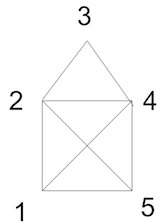
\includegraphics{casetta.png}
\end{figure}

In generale, sono dati $N$ vertici, numerati da $1$ a
$N$, e $M$ lati che li collegano. Dati due vertici
$A$ e $B$, dovete indicare la sequenza di lati
(vanno presi tutti!) da attraversare in modo da collegare $A$
a $B$ passando attraverso tutti i lati nell'ordine indicato
dalla sequenza (senza alzare quindi la matita). Ciascun lato deve
essere percorso una sola volta, in una delle due direzioni a scelta.


\section*{Dati di input}

Il file \texttt{input.txt} è composto da $M+1$
righe. La prima riga contiene quattro interi $N$,
$M$, $A$ e $B$ separati da uno spazio: il
numero di vertici, il numero di lati che li collegano, il vertice di
partenza e quello di arrivo. Le successive $M$ righe
contengono i lati, un lato per riga che viene rappresentato da una
coppia di interi separati da uno spazio (dove i due interi sono i numeri dei vertici collegati da tale lato).


\section*{Dati di output}

Il file \texttt{output.txt} è composto da $M$
righe, 
che riportano la sequenza ordinata dei lati da disegnare per andare
da $A$ a $B$, passando come già detto attraverso tutti i lati una e una sola volta.
Se un lato collega due vertici $X$ e $Y$, deve
essere stampato (indipendentemente da come e' letto nell'input) come
la coppia di interi $X$ e $Y$ separati da uno spazio
se il lato viene viene percorso da $X$ a $Y$, e come
la coppia di interi $Y$ e $X$ separati da uno spazio
se il lato viene viene percorso da $Y$ a $X$ (vedi esempio).

\section*{Assunzioni}

\begin{itemize}
  \item $1 ≤ N ≤ 100000$
  \item $1 ≤ M ≤ 1000000$
  \item $1 ≤ A, B ≤ N$ e $A ≠ B$.
\end{itemize}

\section*{Esempi di input/output}
    \noindent
    \begin{tabular}{p{11cm}|p{5cm}}
    \toprule
    \textbf{File \texttt{input.txt}}
    & \textbf{File \texttt{output.txt}}
    \\
    \midrule
    \scriptsize
    \begin{verbatim}
5 8 1 5
1 4
2 3
5 4
2 1
2 4
3 4
1 5
5 2
\end{verbatim}
    &
    \scriptsize
    \begin{verbatim}
1 2
2 3
3 4
4 5
5 2
2 4
4 1
1 5
\end{verbatim}
    \\
    \bottomrule
    \end{tabular}


\section*{Nota/e}

\begin{itemize}
  \item Viene garantito che sia sempre possibile disegnare senza alzare la matita. Nel caso vi siano più soluzioni valide, è sufficiente restituirne una.
  \item Non esistono lati multipli che collegano la stessa coppia di vertici. Tutti i vertici e tutti i lati devono essere attraversati dalla matita.
  \item Per chi non lo avesse riconosciuto, questo è il noto problema del matematico Eulero.
\end{itemize}

\end{document}
